\def\mySecNum{1.2}
\mySection{\mySecNum~An overview of financial markets}
%-------------- start slide -------------------------------%{{{ 1
\begin{frame}[fragile,t]
	The trading of a financial asset involves at least four discrete steps:
	\bigskip

	\begin{enumerate}
		\item A buyer and a seller must locate one another and agree on a price
			\bigskip
		\item The trade must be \textcolor{magenta}{cleared}\\
			(the obligations of each party are specified)
			\bigskip
		\item The trade must be \textcolor{magenta}{settled} \\
			(the buyer and the seller must deliver the cash or securities necessary to satisfy their
			obligations in the required period of time)
			\bigskip
		\item Ownership records are updated.
	\end{enumerate}
	\vfill

	\begin{center}
		\begin{tikzpicture}[scale=1, transform shape]
		\tikzset{>=latex}
		\only<1->{\node[draw] (1) at (0,0) {Striking a price};}
		\only<2->{\node[circle,draw] (2) at (2.7,0) {clearing};
			\draw[->, shorten <= 0.3em, shorten >= 0.3em] (1) -- (2);}
		\only<3->{\node[circle,draw] (3) at (5,0) {settling};
			\draw[->, shorten <= 0.3em, shorten >= 0.3em] (2) -- (3);}
		\only<4->{\node[draw] (4) at (8,0) {maintaining records};
			\draw[->, shorten <= 0.3em, shorten >= 0.3em] (3) -- (4);}
		\end{tikzpicture}
	\end{center}
\end{frame}
%-------------- end slide -------------------------------%}}}
%-------------- start slide -------------------------------%{{{ 1
\begin{frame}[fragile,t]
	There are at least four different \textcolor{cyan}{measures of a market and its activity}:
	\bigskip
	\begin{enumerate}
		\item \textcolor{magenta}{Trading volume}: the number of financial claims that change hands
			daily or annually.  \bigskip
		\item \textcolor{magenta}{Market value or market cap}: the sum of the market value of the claims
			that \textcolor{cyan}{could} be traded, without regard to whether they have traded.
			\bigskip
		\item \textcolor{magenta}{Notional value}: Notional value measure the scale of a position,
			usually with reference to some underlying asset.
			\bigskip
		\item \textcolor{magenta}{Open Interest}. Open interest measures the total number of contracts
			for which counter parties have a future obligation to perform. It is an important statistic in
			derivatives market.
	\end{enumerate}
\end{frame}
%-------------- end slide -------------------------------%}}}
%-------------- start slide -------------------------------%{{{ 1
\begin{frame}[fragile,t]

\begin{center}
	Companies typically raise funds by
	\bigskip
	\bigskip

	\renewcommand{\arraystretch}{1.2}
	\begin{tabular}{|c|c|}
		\hline
		\textcolor{magenta}{stock markets} & \textcolor{cyan}{bound markets}         \\
		\hline
		Selling ownership claims           & Obtaining a bank loan or issuing a bond \\
		Securities exchanges               & Through dealers                         \\
		(NYSE, NASDAQ)                     &                                         \\
                                       & less frequent                           \\
	  \hline
	\end{tabular}
\end{center}
\end{frame}
%-------------- end slide -------------------------------%}}}
%-------------- start slide -------------------------------%{{{ 1
\begin{frame}[fragile,t]
	The introduction of derivatives in a market often coincides with \textcolor{magenta}{an increase
	in price risk} in that market. For example,
\begin{enumerate}
	\item Currencies were permitted to float in 1971 when the gold standard was officially abandoned.
		The modern market in financial derivatives began in 1972, when the \textcolor{cyan}{Chicago
		Mercantile Exchange} started trading futures contracts on seven currencies.
	\item OPEC’s 1973 reduction in the supply of oil was followed by high and variable oil prices.
	\item U.S. interest rates became more volatile following inflation and recessions in the 1970s.
	\item The market for natural gas has been deregulated gradually since 1978, resulting in a
		volatile market in recent years.
	\item The deregulation of electricity began during the 1990s.
\end{enumerate}
\end{frame}
%-------------- end slide -------------------------------%}}}
%-------------- start slide -------------------------------%{{{ 1
\begin{frame}[fragile,t]
	\begin{center}
	History of the crude oil prices  \bigskip \bigskip

	\includegraphics[scale=0.25]{figs/crude-oil-price-history-chart-neg.png}\footnote{Image from
	\url{https://www.macrotrends.net/}}
	\bigskip

	\end{center}
\end{frame}
%-------------- end slide -------------------------------%}}}
%-------------- start slide -------------------------------%{{{ 1
\begin{frame}[fragile,t]

\begin{center}
 Price variability leads to the development of derivatives markets to efficiently share risk.
 \bigskip \bigskip

 \includegraphics[scale=0.3]{figs/Figure1-1-d.png}
 \bigskip

 Millions of future contracts traded annually at the Chicago Board of Trade (CBT), Chicago
 Mercantile Exchange (CME), and the New York Mercantile Exchange (NYMEX), 1970-2011.
\end{center}
\end{frame}
%-------------- end slide -------------------------------%}}}
%-------------- start slide -------------------------------%{{{ 1
\begin{frame}[fragile,t]
\begin{center}
	Examples of underlying assets on which futures contracts are traded: \bigskip

	\includegraphics[scale=0.25]{figs/Table1-2.png}
\end{center}
\end{frame}
%-------------- end slide -------------------------------%}}}
%-------------- start slide -------------------------------%{{{ 1
\begin{frame}[fragile,t]
	\frametitle{The role of financial markets}
	\begin{center}
	Insurance companies and individual communities/families have traditionally helped each other to share risks.
	\pause
	\bigskip
	\mySeparateLine
	\bigskip

	Markets make \textcolor{alert}{RISK-SHARING} more efficient \\
	\bigskip
	\renewcommand{\arraystretch}{1.2}
	\begin{tabular}{c|c|c}
		\textcolor{magenta}{Diversifiable risks}  & vanishes                 & lightening strike  \\
		\textcolor{cyan}{Non-diversifiable risks} & are reallocated to those & Stock market crash \\
                                              & most willing to hold it  &                    \\
	\end{tabular}
	\bigskip
	\bigskip
	\pause

	The existence of risk-sharing mechanisms benefits everyone!
	\end{center}
\end{frame}
%-------------- end slide -------------------------------%}}}
